\section{Off Product Inspector Tooling}

  The Off Product Inspector (OPI) was made so that people in editorial and partner marketing and non technical team members, could view the data that
  should be available to partners at that moment. It allows users to search for pids (unique identifiers) and titles of brands, series and episodes
  and then view the data of these items. I worked on two main things to extend this project, upgrade to support our new v2 catalogues and add the 
  Deeplink Generator.

  \subsection{Support v2 Catalogues}
  The OPI originally was designed to support the v1.1 catalogue, however the catalogue had been extended to v2 which included different data and also 
  had 3 \textit{horizon catalogues}.
  \begin{itemize}
    \item \textbf{v2.0 catalogue} - Contains all data, both what is currently available and unavailable on iPlayer.
    \item \textbf{v2.0 0-day catalogue} - Contains data that is on iPlayer right now.
    \item \textbf{v2.0 8-day catalogue} - Contains data that is on iPlayer right now and also contains things that will be available within 8 days.
  \end{itemize}

  Partners are being encouraged to move over to the new v2 version of the catalogue so its good to be able to see what theses catalogue should offer.
  Me and a fellow junior software engineer began by working on the \textit{spike} for the project. A spike is a task thats aim is to gain knowledge
  \todo[noline, size=\small]{B5}
  and information on ahead of doing the work. This can often times mean creating a small MVP to show that it is possible. I talk about this and other
  software lifecycle issues in the \textbf{Software Engineering-1.pdf} document. The spike we created was an MVP that allowed the switching between 
  catalogues, however the code was not refined, there was no tests written and zero documentation, this would all come later. We then showed what we 
  had come up with to the team and then began the process of breaking the work down into slices/tickets.

  \vspace{0.2cm}

  I had never done or heard of a \textit{spike} before doing this for the OPI. It's easy to get carried away and go beyond the scope of the spike.
  Towards the end of this spike I began writing some tests for certain things but learned that this was not part of what a spike was. When doing 
  another spike for the schedules ingester, I took this lesson and stayed within the scope. \todo[noline, size=\small]{L2, L3, L7, L8}

  \subsection{Working across teams}
  As this was a web app, it required a UI (user interface). We also needed to speak to the stakeholders/users to understand what they use the tool 
  for. We had meetings in which we as a team were joined by people from the UI/UX team, as well as the user, Editorial and Partner Marketing. In 
  these meetings we discussed what data we had and what the users wanted to see, all whilst UX took notes for a later design. We didn't
  technically need a UX design, however this was a tool to be used by non-developers and therefore required more finesse than devs would have at
  displaying the information in a readable, understandable way. We set up a separate Slack channel for UX discussions so that changes and 
  alterations could be made as the project progressed.

  \todo[noline, size=\small]{B3, L6}

  I think the creation of a separate Slack channel for communication throughout the project was great and let us make subtle changes to the UI
  as new things came to light. These meetings were also extremely helpful and brought to light some other ideas like the 
  \textbf{Deeplink Generator}, which was then created to help another team further down the line. SpaceChimp is somewhat at the end of the line 
  as we are the final thing before partners receive their data, this can lead to us not working with other teams too much. I think this project 
  highlights that we can still work with other teams to enable them in their jobs more. 
  
  We then worked with UX again for the Deeplink Generator, where we added images to the initial UI/UX to add more colour to the page.


  This is an area I have much more knowledge in from my own teachings and allowed me to help/teach my colleague I was spiking with learn
  about how things like React hooks work and the interplay between React and Next.js. Throughout my apprenticeship I have paired with colleagues 
  that have more experience than me. Pairing is when two developers work together on a task, one writes the code whilst the other observes. This is great 
  \todo[noline, size=\small]{L8}
  for learning as the one with less experience can get feedback instantly on what they're doing and ask for help. It's important to let the learner 
  do most of the coding as this helps them get to grips with what's going and think more. If it was the other way they may not understand what is 
  happening, or it the code may be written to quickly for them to understand what is being done. This is also a good time to gey to know other 
  members of the team. Especially in a remote setting, it can be easy to program alone with minimal interaction, pairing helps to promote 
  relationships and conversations within the team.

  Further along in the project I also suggested that we move to a newer way of writing css and components called \textit{styled components}. Some benefits of
  these are:
  \todo[noline, size=\small]{T2, L3}
  \begin{itemize}
    \item Styles are not separate from the component itself, making it easier to debug.
    \item Styled components can take props to easily customise aspects of a components style.
    \item Default html tags are given a more meaningful name, making it easier to understand the role of a tag.
  \end{itemize}

  Below is an example of the difference between using styled components and styling using SaSS (Syntactically Awesome Style Sheets).

  \begin{figure}[H]
    \centering
    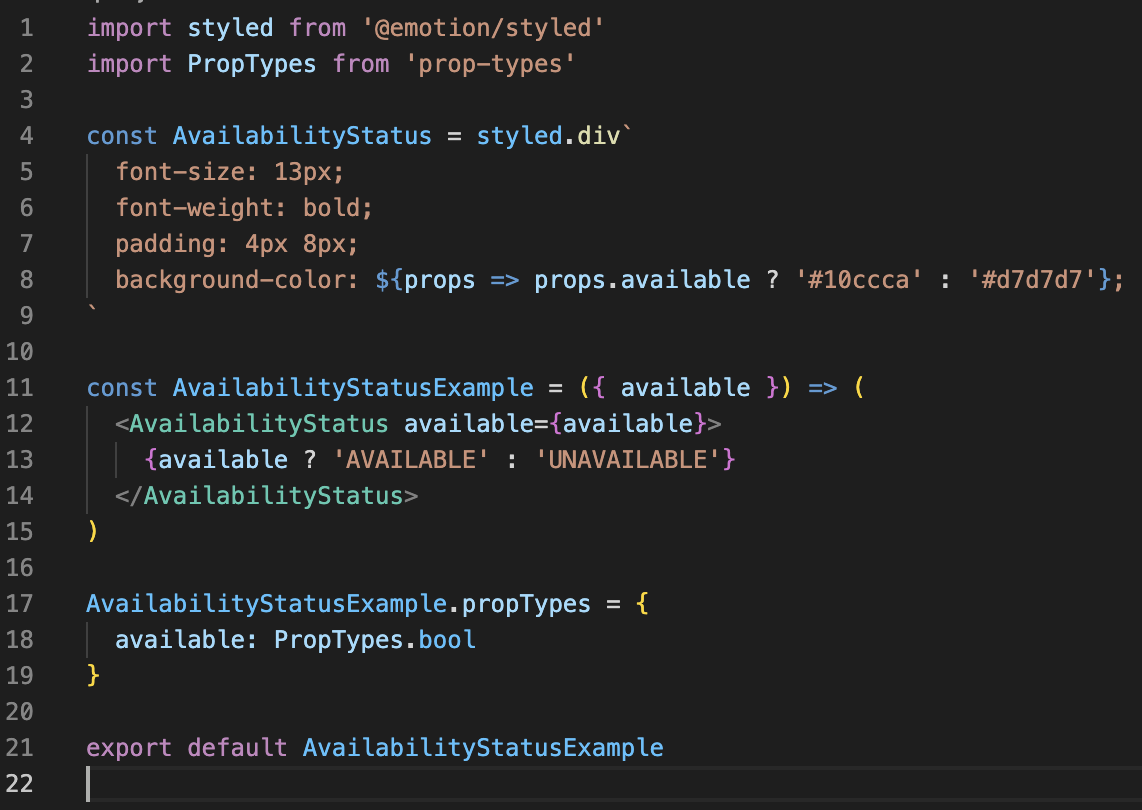
\includegraphics[width=6cm, height=4cm]{assets/StyledCompsOldJSX.png}
    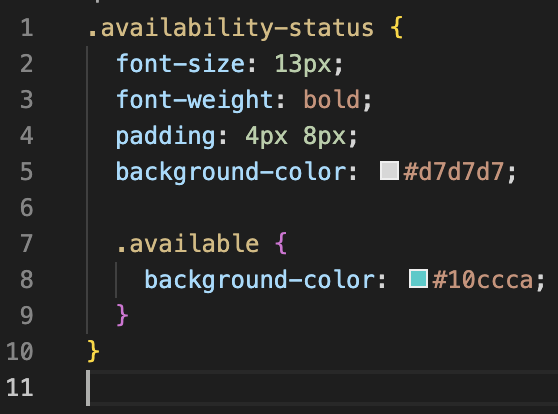
\includegraphics[width=6cm, height=4cm]{assets/styledCompsOldCSS.png}
    \caption{Screenshots of how not using styled components would work, JSX on left, SCSS on right.}
    \label{fig:oldStyling}
  \end{figure}

  \begin{figure}[H]
    \centering
    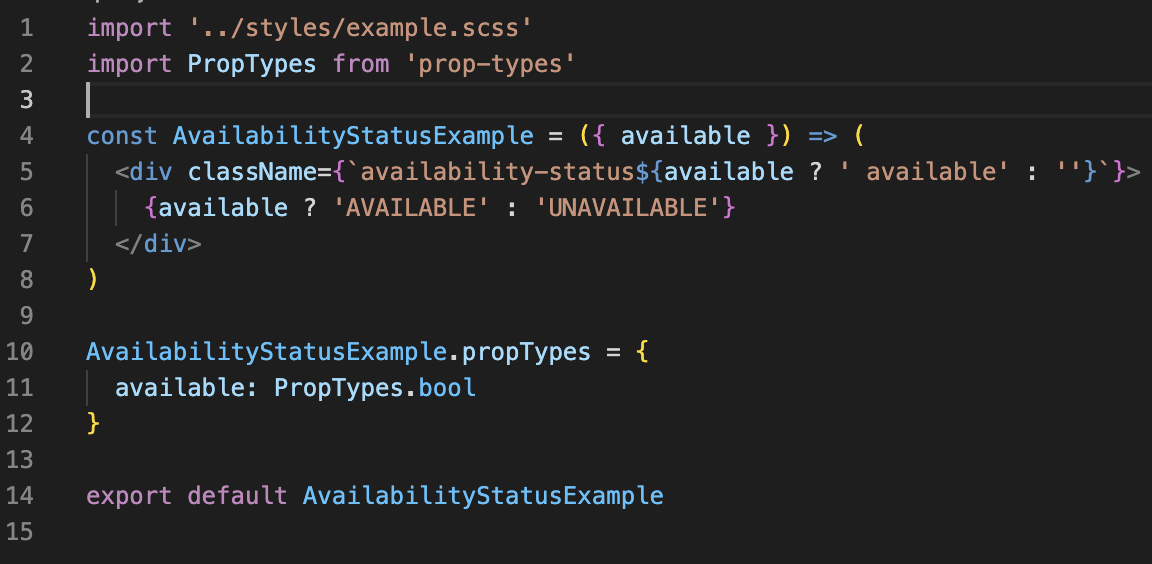
\includegraphics[width=8cm]{assets/styledCompsNew.png}
    \caption{Screenshot of how it looks using styled components.}
    \label{fig:newStyling}
  \end{figure}

  \subsection{Deeplink Generator}
  Deeplink generator stuff here.

    \subsubsection{Deeplink Generator Presentation}
    \todo[noline, size=\small]{P2}
    On the 18th of July 2023 I presented at the Partnerships show n' tell meeting on behalf of my team. I presented the work we did for the
    deeplink generator and have included the slides in a separate document.

    This was the first time I've presented anything to a larger group of people and I was nervous going in. The presentation was short, due to the work
    being discussed not being very large, however it still took around 5 -7 minutes for the whole presentation. Overall I'm happy with how I managed the 
    presentation and with the presentation itself. It's something I should do more of in the future to become more comfortable with these kinds of things.
    For future I would take my time more when going through the slides. I felt like I rushed a little bit due to my nerves, however I feel like this is 
    something that comes with practice and being the the situation. 

  \subsection{Personal feedback on OPI}
  \todo[noline, size=\small]{P2, L9, L10}
  I show the questions and feedback I received in the document \textbf{Feedback Form Output.docx}. I also go into a discussion of this in the document
  \textbf{Leaderships-1.pdf}.

  Reflecting now (August 2023) on the goals at the end of that assignment:
  \begin{itemize}
    \item \textbf{Pass AWS practitioner foundational} - I think I've outgrown this aim naturally. My skills and understanding of AWS is much greater than
    that of which I'd be assessed on. I am deffinately still interested in gaining some qualifications in AWS, however I would prefer for now to focus on 
    finishing my masters/apprenticeship rather than do that. In the future I will look into doing the develop or solutions architect certifications.
    \item \textbf{Improve input in meetings} - This is something I've got better at, partly due to me learning more about what we do as a team and therefore
    feeling less \textit{'imposter syndrome'} when giving out ideas.
    \item \textbf{Attend BBC mentoring training} - I am currently on the wait-list for this course.
  \end{itemize}

\newpage